\section{Method}

% --- COPIED FROM ABSTRACT ASSIGNMENT --- %
% Explain your study design, illustrate how the study's results will provide
% evidence for/against your hypothesis, and how the question, hypothesis, and
% study all line up. We encourage you to mirror/copy/adapt other researchers
% methods (e.g. by drawing from the class readings) whenever appropriate (and
% not when it isn't appropriate).

% There are three major points you should hit here.

% Study design:
% What are you going to do? Be detailed and precise.

% Ecological Validity:
% Why does your study answer your research question? Why
% does your evaluation address your hypothesis? Make sure your study, and the
% variables you're measuring, properly address the question you are asking.
\subsection{Measures}
For each participant, we measured:
\begin{itemize}
    \item Time-to-correct solution (per task)
    \item Count of incorrect guesses (per task)
    \item Count and type of interpreter queries (across all tasks)
\end{itemize}

The first metric directly tests the hypothesis that examples improve
selection speed, but the result could be misleading if there was also a
change in selection accuracy.
%
Counting incorrect guesses ensures that any such change is captured.
%
Beyond assessing the effectiveness of examples, measuring how often and why
participants used the interactive interpreter provides insight into any
behavior changes that might occur.

\begin{figure*}[t!]
    \centering
    \begin{subfigure}[t]{0.5\textwidth}
        \centering
        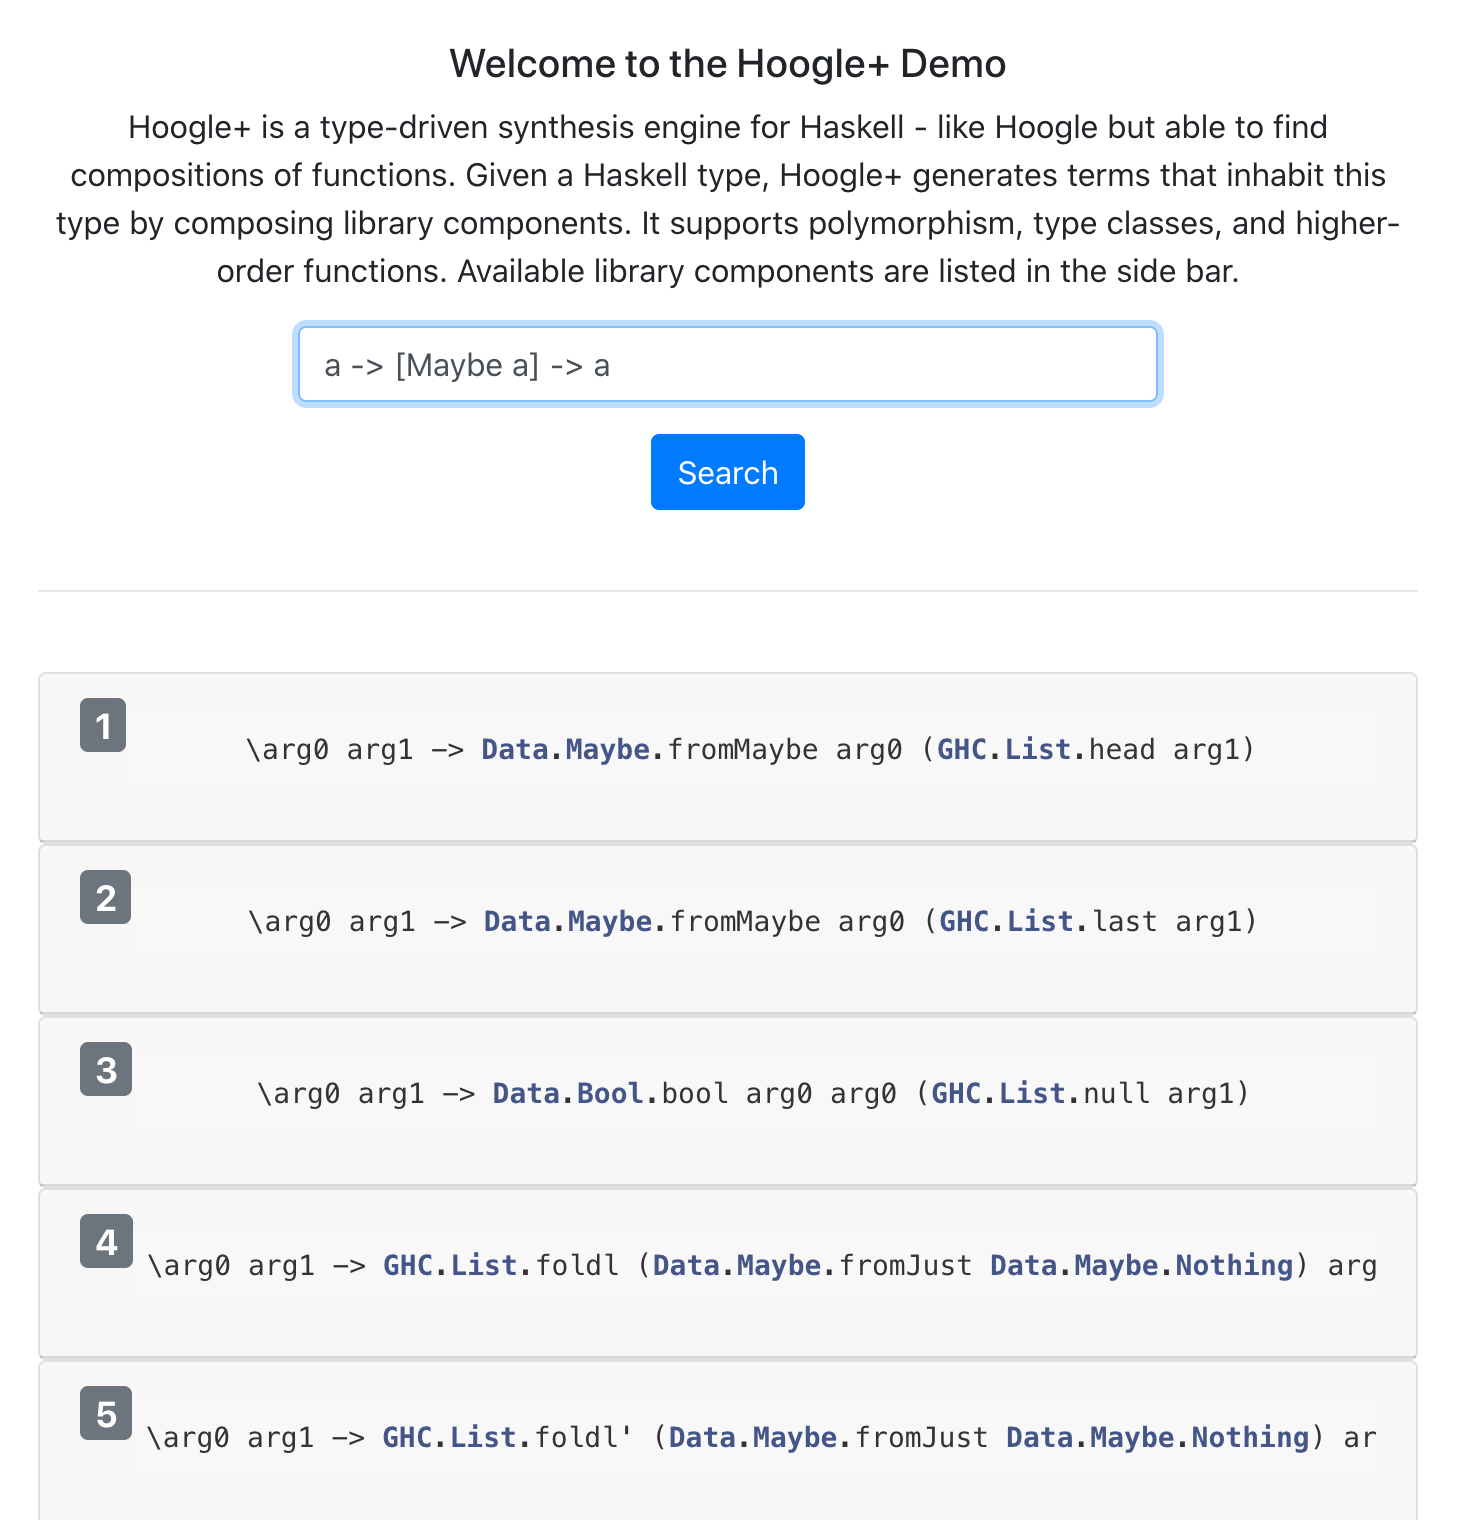
\includegraphics[width=\textwidth]{method/control-ui.png}
        \caption{Control treatment, no examples}
    \end{subfigure}%
    ~
    \begin{subfigure}[t]{0.5\textwidth}
        \centering
        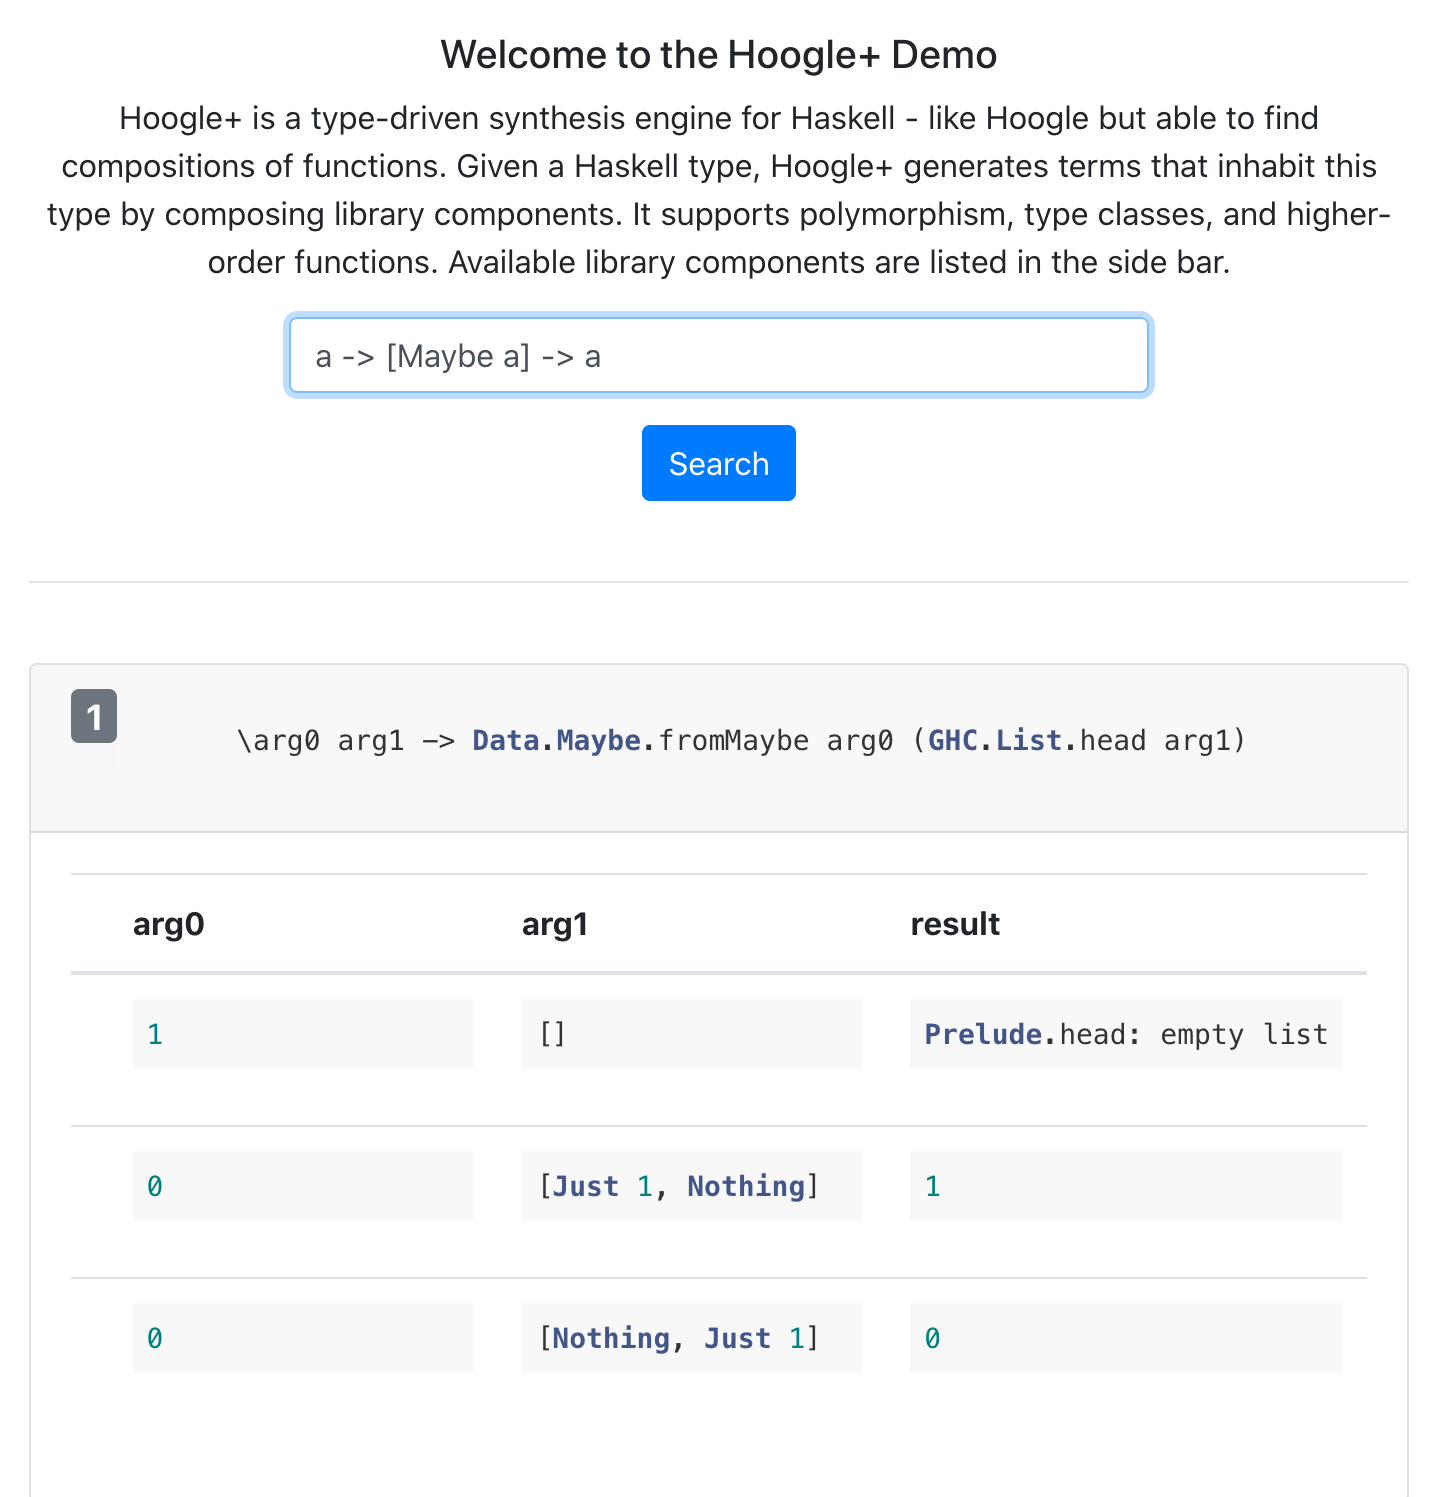
\includegraphics[width=\textwidth]{method/treatment-ui.png}
        \caption{Experimental treatment, examples}
    \end{subfigure}
    \caption{Each participant received one of the two treatments for the duration of the study.}
\end{figure*}